


\documentclass[11pt,titlepage,twoside]{article}\usepackage[]{graphicx}\usepackage[table]{xcolor}
% maxwidth is the original width if it is less than linewidth
% otherwise use linewidth (to make sure the graphics do not exceed the margin)
\makeatletter
\def\maxwidth{ %
  \ifdim\Gin@nat@width>\linewidth
    \linewidth
  \else
    \Gin@nat@width
  \fi
}
\makeatother

\definecolor{fgcolor}{rgb}{0.345, 0.345, 0.345}
\newcommand{\hlnum}[1]{\textcolor[rgb]{0.686,0.059,0.569}{#1}}%
\newcommand{\hlsng}[1]{\textcolor[rgb]{0.192,0.494,0.8}{#1}}%
\newcommand{\hlcom}[1]{\textcolor[rgb]{0.678,0.584,0.686}{\textit{#1}}}%
\newcommand{\hlopt}[1]{\textcolor[rgb]{0,0,0}{#1}}%
\newcommand{\hldef}[1]{\textcolor[rgb]{0.345,0.345,0.345}{#1}}%
\newcommand{\hlkwa}[1]{\textcolor[rgb]{0.161,0.373,0.58}{\textbf{#1}}}%
\newcommand{\hlkwb}[1]{\textcolor[rgb]{0.69,0.353,0.396}{#1}}%
\newcommand{\hlkwc}[1]{\textcolor[rgb]{0.333,0.667,0.333}{#1}}%
\newcommand{\hlkwd}[1]{\textcolor[rgb]{0.737,0.353,0.396}{\textbf{#1}}}%
\let\hlipl\hlkwb

\usepackage{framed}
\makeatletter
\newenvironment{kframe}{%
 \def\at@end@of@kframe{}%
 \ifinner\ifhmode%
  \def\at@end@of@kframe{\end{minipage}}%
  \begin{minipage}{\columnwidth}%
 \fi\fi%
 \def\FrameCommand##1{\hskip\@totalleftmargin \hskip-\fboxsep
 \colorbox{shadecolor}{##1}\hskip-\fboxsep
     % There is no \\@totalrightmargin, so:
     \hskip-\linewidth \hskip-\@totalleftmargin \hskip\columnwidth}%
 \MakeFramed {\advance\hsize-\width
   \@totalleftmargin\z@ \linewidth\hsize
   \@setminipage}}%
 {\par\unskip\endMakeFramed%
 \at@end@of@kframe}
\makeatother

\definecolor{shadecolor}{rgb}{.97, .97, .97}
\definecolor{messagecolor}{rgb}{0, 0, 0}
\definecolor{warningcolor}{rgb}{1, 0, 1}
\definecolor{errorcolor}{rgb}{1, 0, 0}
\newenvironment{knitrout}{}{} % an empty environment to be redefined in TeX

\usepackage{alltt}
\usepackage[a4paper, inner=1.5cm, outer=1.5cm, top=2cm, bottom=3cm]{geometry}

\usepackage[utf8]{inputenc} 
\usepackage[T1]{fontenc}
\usepackage[sort&compress]{natbib}
\usepackage[french]{babel}

\addto\captionsfrench{\def\tablename{Tableau}}
\addto\captionsfrench{\renewcommand*{\contentsname}{Sommaire:}}
\addto\captionsfrench{%
  \renewcommand{\listfigurename}{Liste des figures:}%
  \renewcommand{\listtablename}{Liste des tableaux:}%
  \renewcommand{\abstractname}{Résumé}%
}
\usepackage{caption}
\usepackage[labelsep=endash]{caption}
\usepackage{graphicx}
\usepackage{colortbl}
\usepackage{booktabs}
\usepackage{longtable}
\usepackage{array}
\usepackage{multirow}
\usepackage{wrapfig}
\usepackage{float}
\usepackage{pdflscape}
\usepackage{tabu}
\usepackage{threeparttable}
\usepackage{threeparttablex}
\usepackage[normalem]{ulem}
\usepackage{makecell}
\usepackage[table]{xcolor}
\usepackage{ae,aeguill}
\usepackage{subcaption}

\usepackage{authblk}
\renewcommand\Authand{ et }
\renewcommand\Authands{ et }

\usepackage{textcomp}
\usepackage{hyperref}
\pdfstringdefDisableCommands{%
  \def\\{}%
  }
\hypersetup{ 
colorlinks=true, 
linkcolor=blue, 
citecolor=blue, 
filecolor=blue, 
urlcolor=blue, 
pdftitle= {Suivi et estimation du recrutement en anguille européenne sur le fleuve Seine\\ Année 2024 }, pdfauthor={Marangoni Lucas},
pdfsubject={stacomi},
 pdfkeywords={stacomi} {migrateurs} {Seine} {poissons}
}
\pdfoptionpdfminorversion=7
\renewcommand{\sectionmark}[1]{\markboth{}{\emph{\thesection~#1}}}
\renewcommand{\subsectionmark}[1]{\markboth{}{\emph{\thesubsection~#1}}}
\renewcommand{\subsubsectionmark}[1]{\markboth{}{\emph{\thesubsection~#1}}}

\makeatletter
    \def\@@and{et}
\makeatother

\usepackage{fancyhdr}
\pagestyle{fancy}
\fancyhf{}
\rhead{\rightmark}
\lfoot{\footnotesize{Suivi et estimation du recrutement en anguille européenne sur le fleuve Seine, année 2024}} %Insere un pied de page avec le texte a gauche.
\rfoot{\thepage}
\setlength{\headheight}{15pt}

\usepackage{pdfpages}
\usepackage{setspace}

%%%%%%%%%%%%%%%%%%%%%%%%%%%%%%%%%%%%%%%%%%%
%%%%%% CHUNK DE CHARGEMENT INITIAL  %%%%%%%
%%%%%%%%%%%%%%%%%%%%%%%%%%%%%%%%%%%%%%%%%%%



%% Makes a path to your graphics' folder.
\graphicspath{{image/}}

\title{Suivi et estimation du recrutement en anguille européenne sur le fleuve Seine,
année 2024}

\author[1]{Marangoni Lucas}
\affil[1]{Seine-Normandie Migrateurs, 11 cours Clemenceau 76100 Rouen}
\IfFileExists{upquote.sty}{\usepackage{upquote}}{}
\begin{document}

\hypersetup{pageanchor=false}

\begin{titlepage}

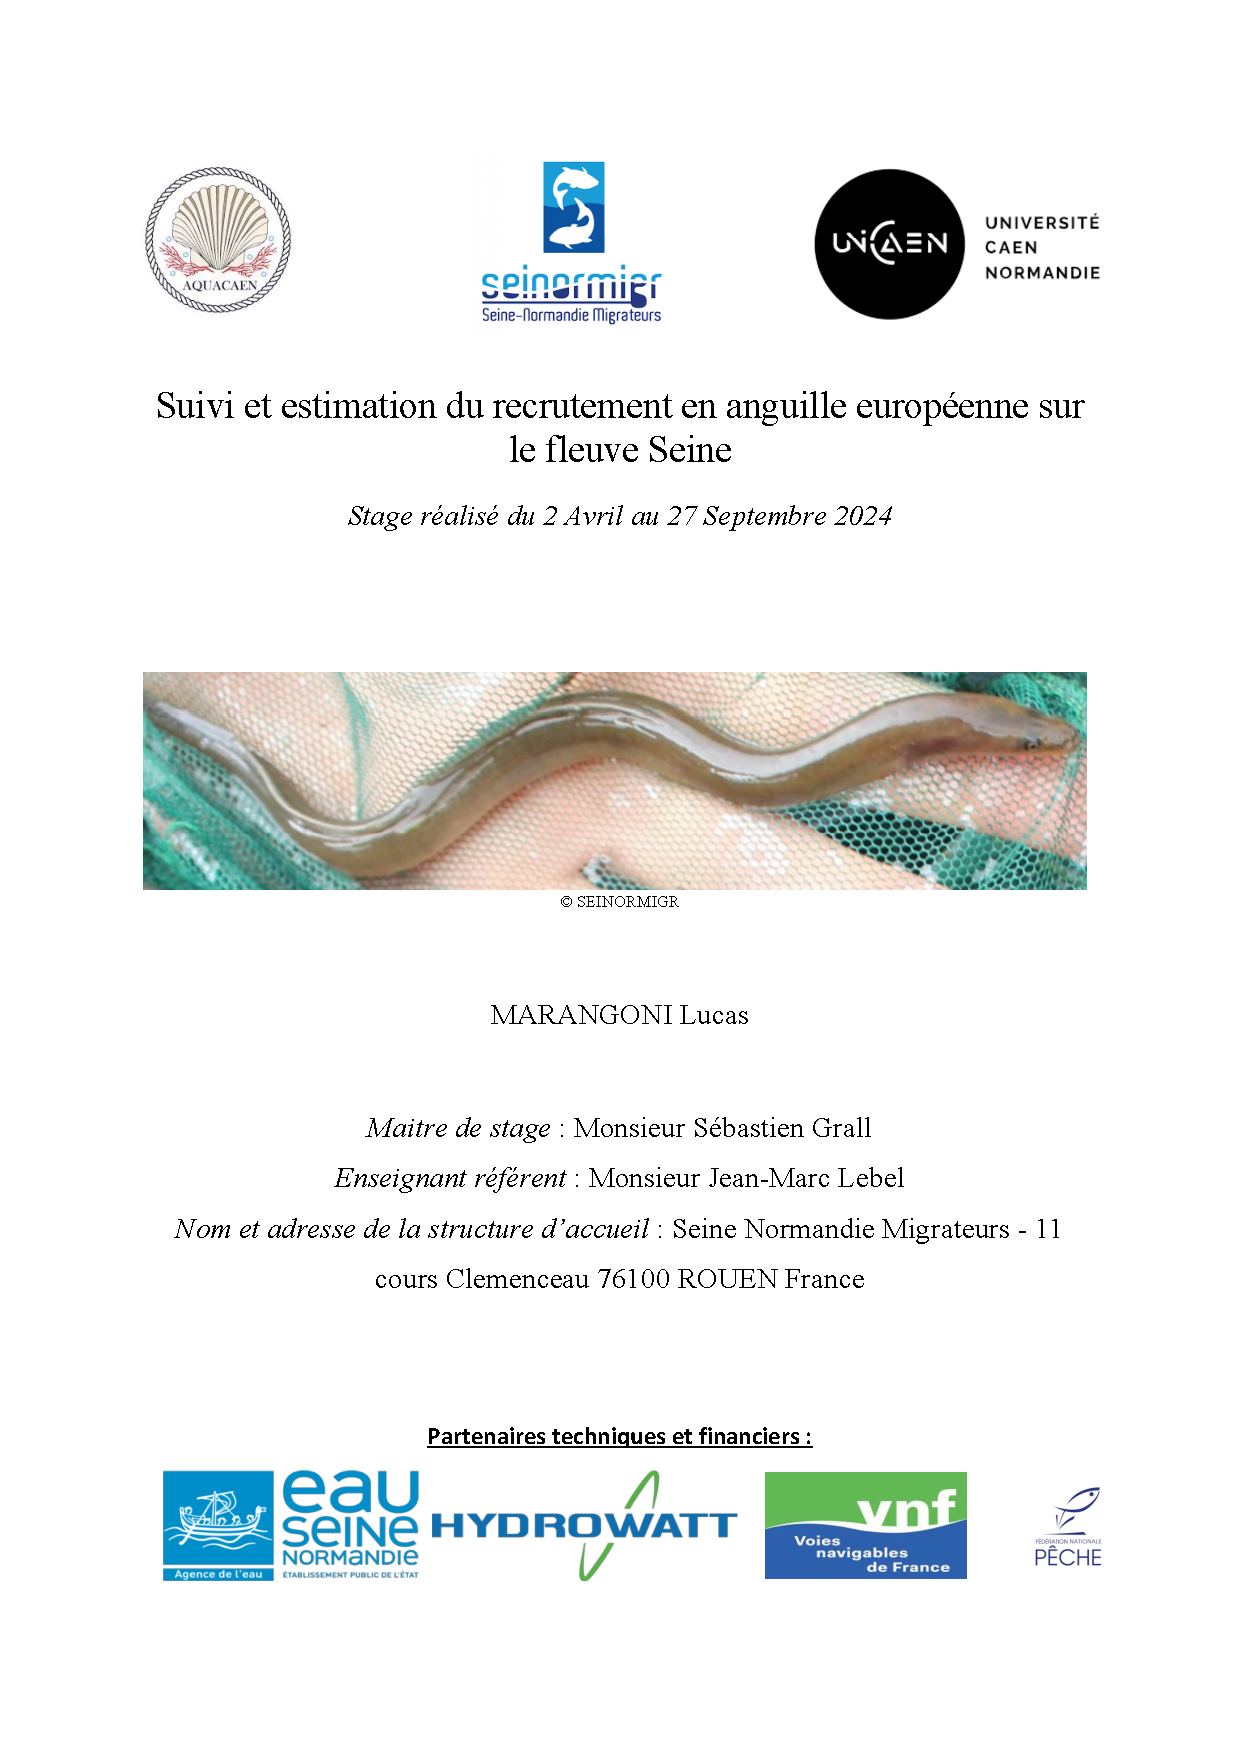
\includepdf[pages=-]{frontpage.pdf}

\end{titlepage}



\newpage
\thispagestyle{empty}
\strut
\newpage

\pagenumbering{roman} \setcounter{page}{1}

\maketitle

\begin{abstract}


Un suivi du recrutement de l’anguille européenne en Seine est réalisé depuis 2014 en rive gauche et 2018 en rive droite du barrage de Poses, premier ouvrage sur la Seine. Ce suivi a été mis en place dans le cadre du Plan National de Gestion Anguille (PGA). Pour cette année 2024, un total de 844 326 anguilles a été comptabilisé avec 86,6\% des individus en rive droite et 13,4\% des individus en rive gauche. La mise en place d’une rampe à anguille en rive droite a fortement augmenté les chiffres car l’accessibilité de la rampe en rive gauche est trop difficile à cause des courants issus de l’usine hydroélectrique. Les facteurs environnementaux jouent un rôle dans la montaison des anguilles. Cette année les résultats ont réussi a montré un impact significatif positif des températures de l’air et de l’eau fortement corrélées entre elles. Les débits et les niveaux d’eau étaient extrêmement élevés, cela a joué un rôle dans l’accessibilité des anguilles en venant modifier et contrer les courants de l’usine hydroélectrique. En complémentarité des dispositifs de piégeages, des flottangs ont été mis en place en aval des rampes visant à vérifier le bon fonctionnement des dispositifs. Une amélioration des chiffres est visible cette année mais nous ne pouvons pas qualifier la situation de satisfaisante comparé aux chiffres des années 80.
Mots-clés :  Anguilla Anguilla ; Montaison ; Recrutement ; Rampe à anguille ; Seine


\end{abstract}

\newpage

\tableofcontents

\clearpage

\listoffigures

\listoftables

\hypersetup{pageanchor=false}

\clearpage

\pagenumbering{arabic} \setcounter{page}{1} 

\clearpage

\begin{center}
\textbf{Seine Normandie Migrateurs}
\end{center}

Préambule : Les informations présentées ci-dessous sont tirées de site internet : https://www.seinormigr.fr. 
\vspace{1cm}

\underline{Présentation générale} : Seinormigr a été créé en 2007 sur une initiative du Président de la Fédération de la Seine-Maritime pour la Pêche et la Protection du Milieu Aquatique. 
L’association regroupe par adhésion les Fédérations départementales présentes sur le bassin Seine-Normandie afin de créer une seule et même continuité dans le suivi et la gestion des populations de poissons migrateurs. 
En 2011, elle est inscrite au Plan de Gestion des Poissons Migrateurs du bassin Seine-Normandie où elle siège en tant qu’inviter. 
En 2012, Seinormigr obtient son agrément d’association de protection de l’environnement par arrêté préfectoral du 13 décembre 2012. 
Puis en 2013, l'association est habilitée pour prendre part aux débats environnementaux se déroulant dans le cadre des instances consultatives régionales. 
Enfin en 2020, Seine-Normandie Migrateurs et Normandie Grands Migrateurs ont fusionné pour ne créer qu'une seule association grands migrateurs sur le territoire Seine-Normandie.
\vspace{1cm}

\underline{Missions} :

-	Contribuer à la connaissance, l’évaluation et au suivi des populations piscicoles amphihalines sur le bassin Seine-Normandie et la région Normandie.

-	Favoriser la valorisation et la gestion des grands migrateurs, notamment avec un porter à connaissance technique et scientifique qui soit visible et accessible en veillant au développement durable des pratiques halieutiques.

-	Participer et s’investir techniquement et/ou financièrement dans les projets de restauration des axes de circulation et des habitats de reproduction et de développement des poissons migrateurs en vue d’assurer leur sauvegarde et la recolonisation des cours d’eau.

-	Assister les maîtres d’ouvrages et les services instructeurs en matière technique et administrative dans tous les projets contribuant à l’accomplissement du cycle biologique des grands migrateurs.

-	Mener ou coordonner des études ou publications spécifiques en concertation avec les différents gestionnaires et pouvoir publics en appui aux décisions politiques locales de l’eau afin de démontrer le bénéfice de l’action à consentir à toutes les échelles des cours d’eau.

-	Participer à la définition et la mise en œuvre des objectifs de restauration des populations de poissons migrateurs au sein du COGEPOMI et de son PLAGEPOMI en collaboration étroite avec le secrétariat technique (DRIEE Île de France, Délégation de bassin) et les établissements publics de l’Etat (DREAL, AFB, Agence de l’Eau, DDTM, …).

-	Développer une large communication de synthèse des productions basées sur des données d’expertises, notamment à l’aide de mise à disposition d’outils de communication à différentes échelles des besoins qu’ils soient locaux, régionaux ou de bassins.
\vspace{1cm}

\underline{Territoires d’action} :  Seine Normandie Migrateurs fait partie des 8 associations migratrices présentent en France qui recouvrent les grands bassins français (Figure \ref{AM_National}). 
L’association regroupe par adhésion 18 Fédérations Départementales pour la Pêche et la Protection du Milieu Aquatique (FDAAPPMA), des Associations Agréées pour la Pêche et la Protection du Milieu Aquatique (AAPPMA), ainsi que des adhérents directs. 
Son territoire s’étend sur une superficie totale de 95 500 km², englobant près de 50 000 km de cours d’eau, composé d’une très grande partie du bassin versant de la Seine et de ceux des fleuves côtiers Normands. 

\vspace{1cm}

\begin{figure}[htpb]
\centering
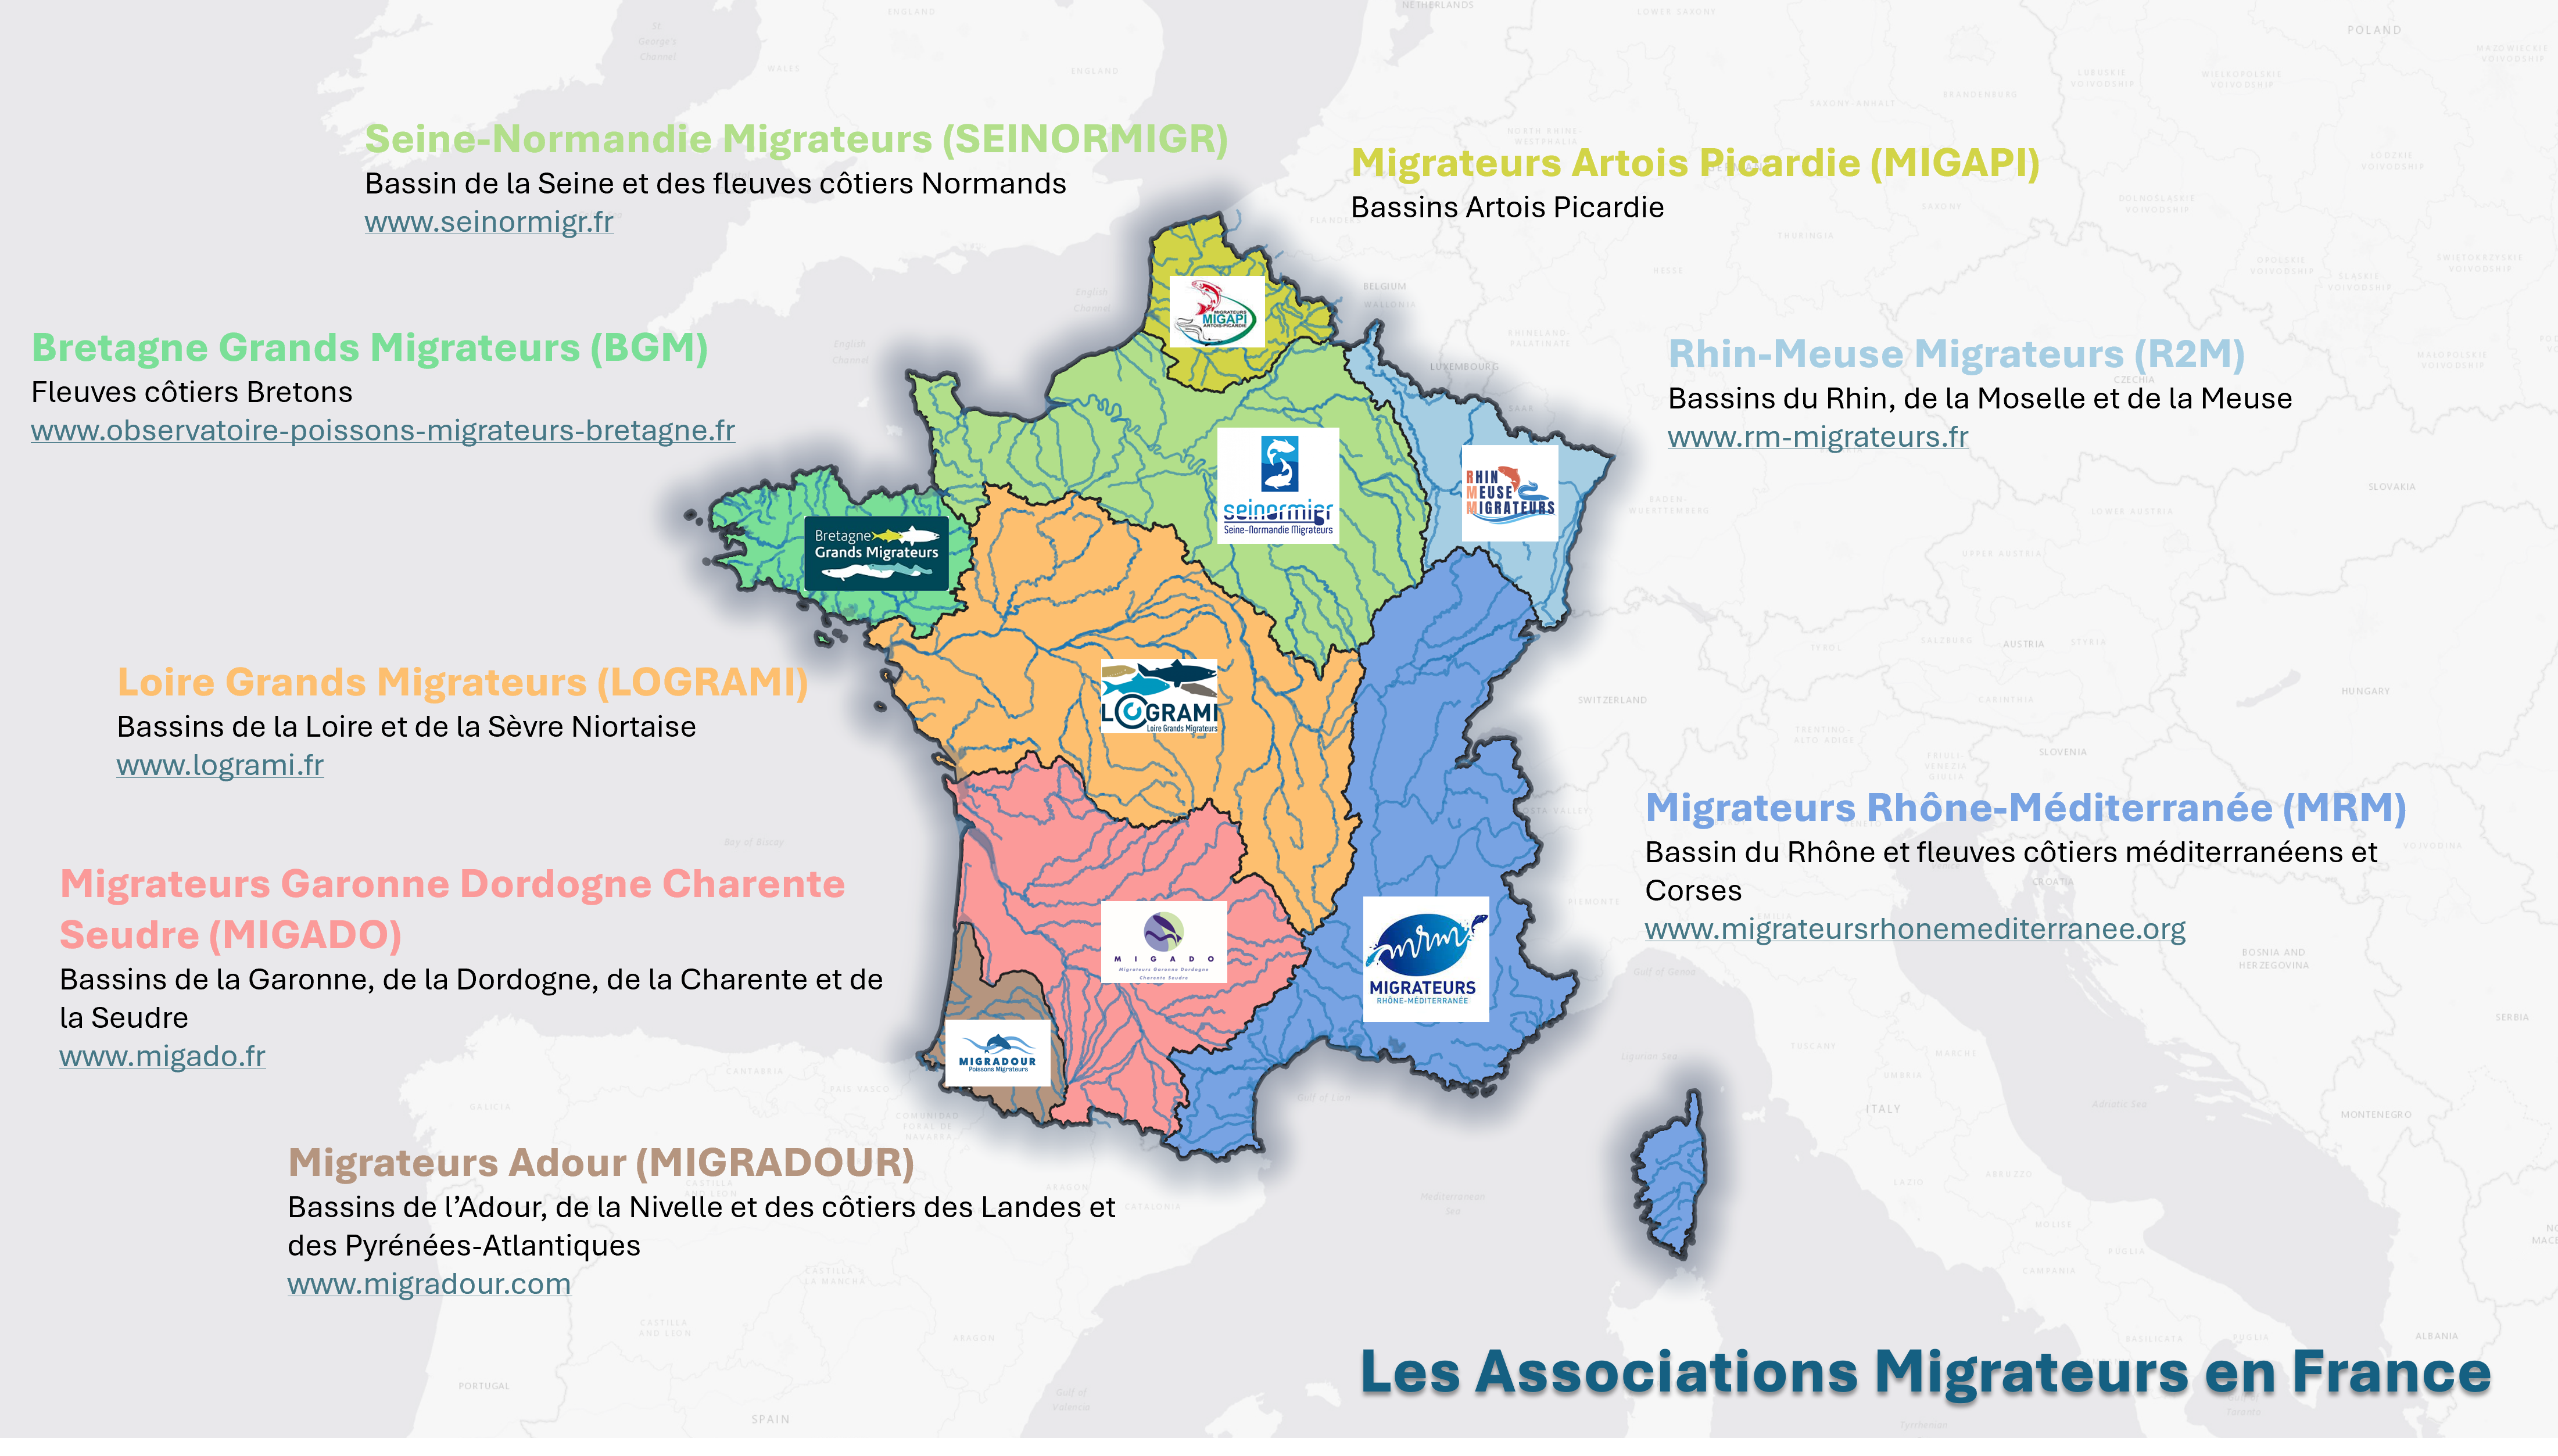
\includegraphics[width=\textwidth]{AM_National.png}
\caption{Associations migrateurs (AM) des grands bassins français (SEINORMIGR)}
\label{AM_National}
\end{figure}


\underline{Organisation} : Plus de 200 000 pêcheurs à travers 18 fédérations départementales pour la pêche et la protection des milieux aquatiques sont représentés par Seinormigr. 
L’association est dirigée par un conseil d’administration de 20 membres avec à sa tête le Président M. Martial CHOUQUET, également président de la FDPPMA de l’Eure. Aujourd’hui l’équipe technique est composée de 6 salariés permanents répartis sur deux antennes Rouen (76) et Mondeville (14) (Figure \ref{Organigramme_Seinormigr}) :

\begin{figure}[htpb]
\centering
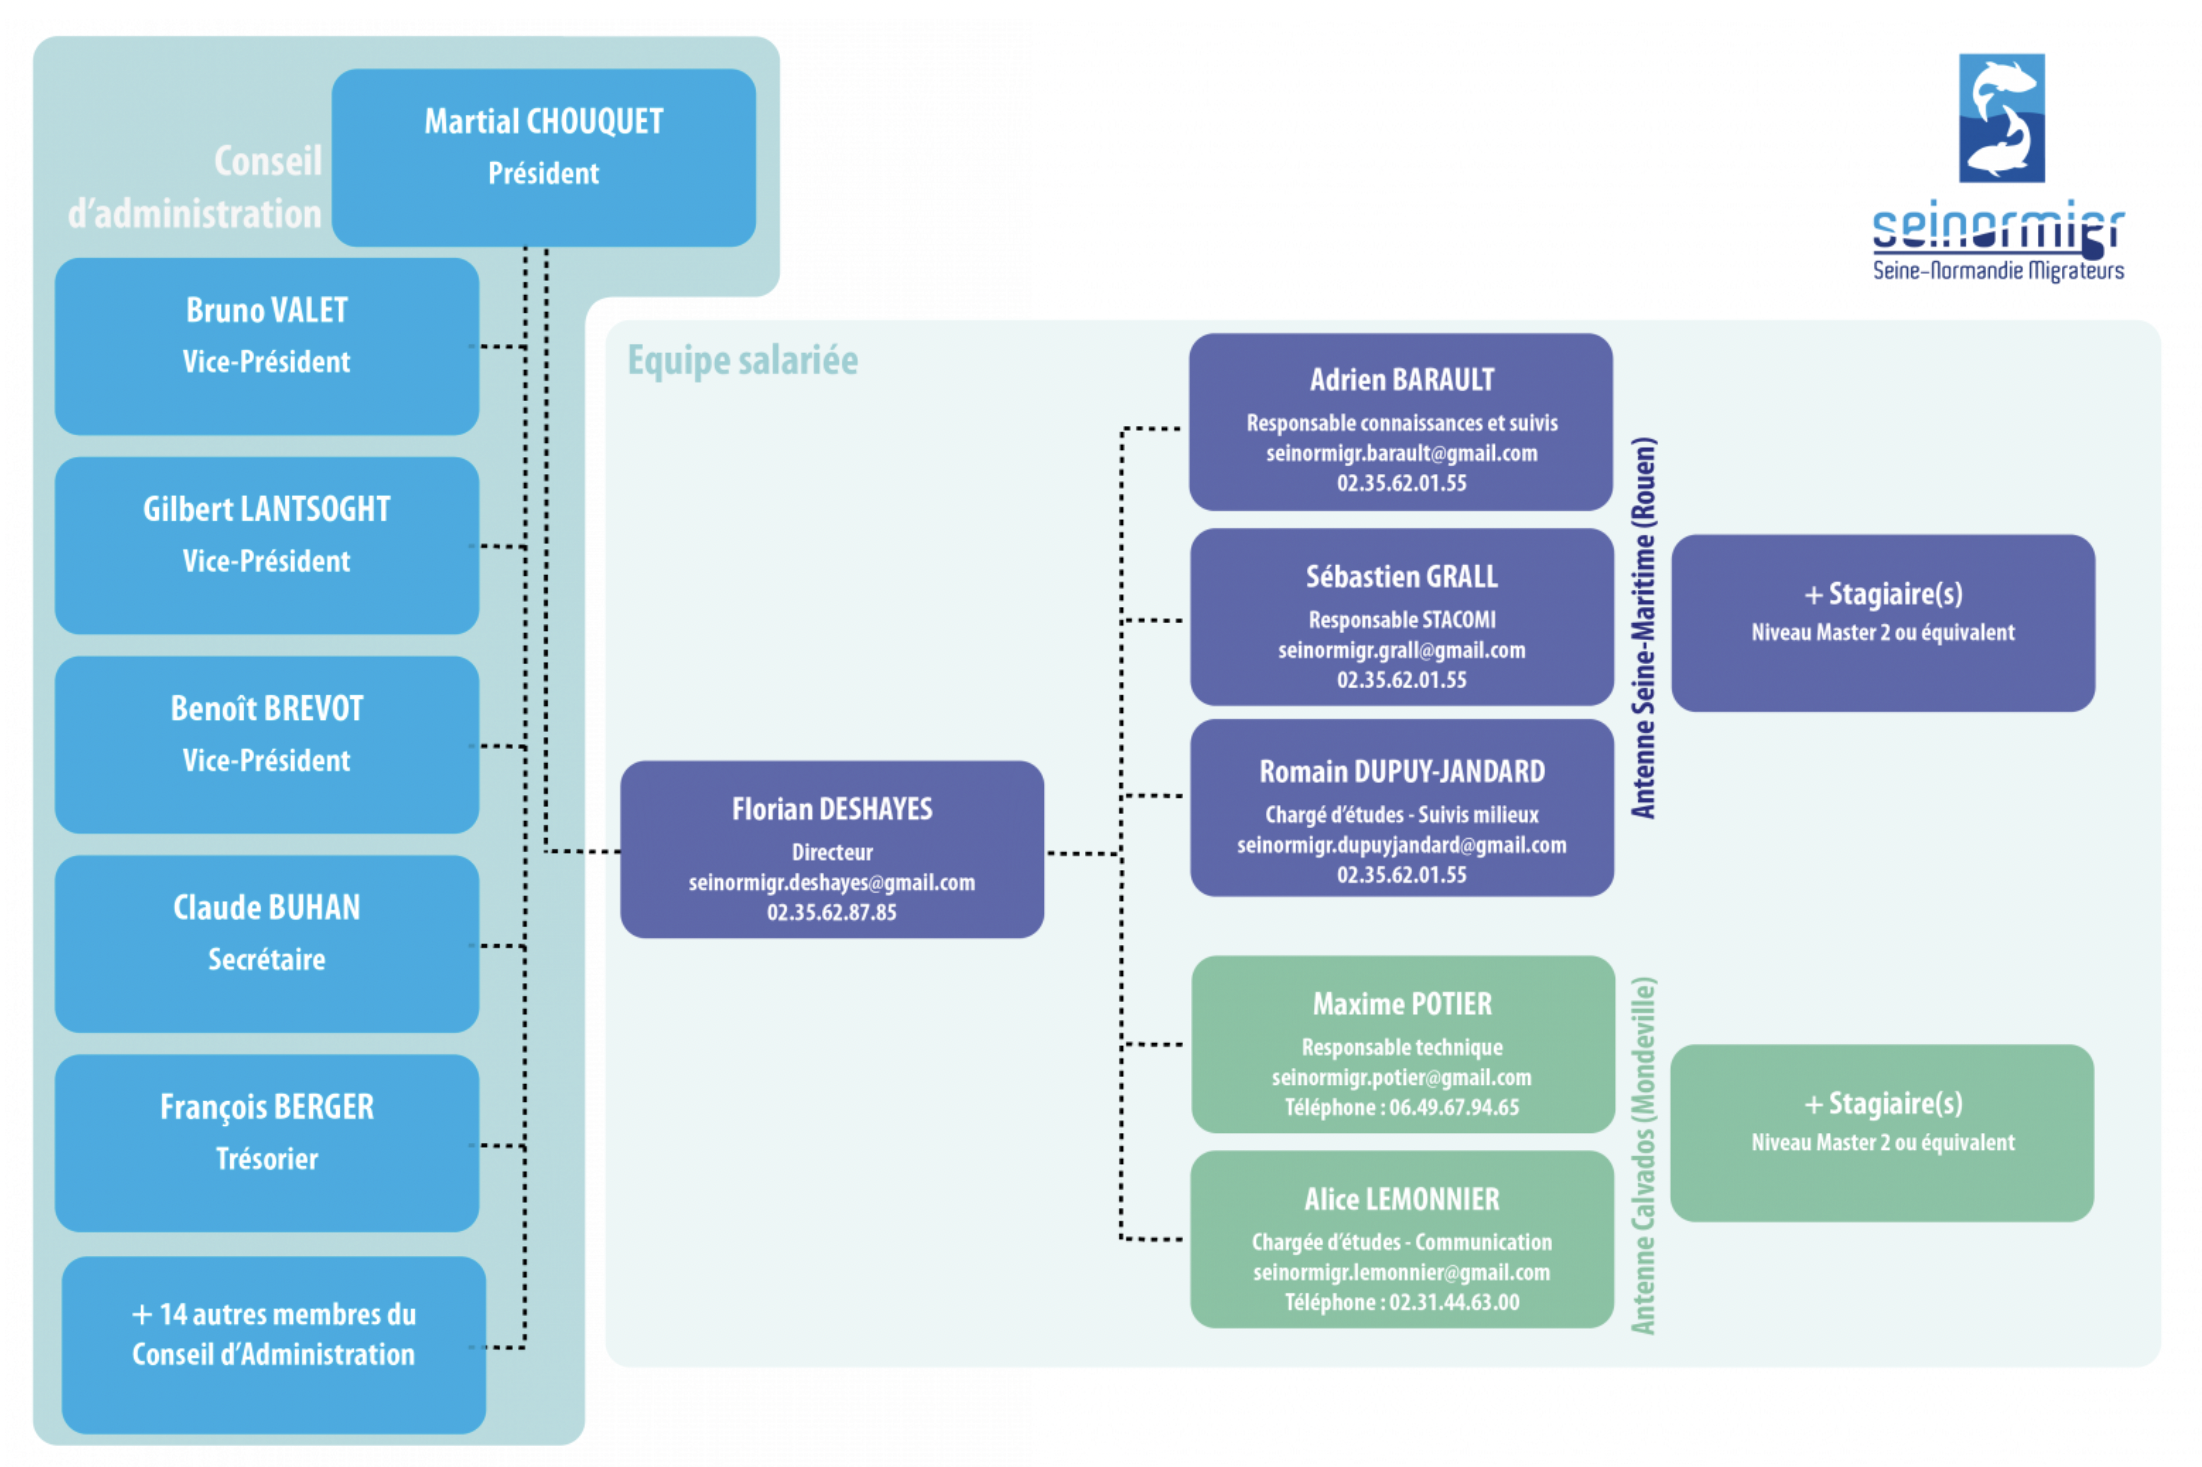
\includegraphics[width=\textwidth]{Organigramme_Seinormigr.png}
\caption{Organigramme de l'association Seinormigr}
\label{Organigramme_Seinormigr}
\end{figure}

-	Florian DESHAYES, Directeur (Rouen)

-	Maxime POTIER, Responsable technique (Mondeville)

-	Adrien BARAULT, Responsable - connaissances/suivis (Rouen)

-	Sébastien GRALL, Responsable - Stations de contrôle des migrations (Rouen)

-	Alice LEMONNIER, Chargée d'études – communication (Mondeville)

-	Romain DUPUY-JANDARD, Chargé d'étude - suivis milieux (Rouen)

\section{Introduction}

\subsection{Contexte historique de l’étude}

Les ecosystemes marins et dulcicoles jouent un role crucial pour l'humanite, fournissant des services essentiels (FAO 2020). 
Cependant, au cours des dernières décennies, l'augmentation rapide des activités anthropiques, telles que l'urbanisation, l'industrialisation, et l'agriculture intensive, a entraîné une dégradation significative de ces environnements naturels (FAO 2020). 
Les activités humaines constituent la 1ère cause d’érosion de la biodiversité mondiale (UICN). 
En France, près de 25\% des poissons dulçaquicoles et amphihalins sont considérés à minima comme menacés (18 espèces sur 80) (UICN, 2019). 
Il est estimé que près d’une espece d’eau douce sur trois est menacée d’extinction (WWF 2020). 

L’anguille européenne est une des espèces qui a été extrêmement touchées par ces menaces (Dekker et Beaulaton, 2016). Autrefois abondante dans les eaux européennes, jugée nuisible jusqu’en 1984, l’espèce représentait plus de 50\% de la biomasse piscicole de l’aval des systèmes fluviaux (Bruslé et Quignard, 2013 ; Moriarty et Dekker, 1997). 
Ensuite, la population d'anguilles a drastiquement diminué depuis le milieu du XXème siècle. Initialement classée comme "vulnérable", elle est ensuite passée à "en danger", pour finalement aujourd’hui atteindre le statut "en danger critique d'extinction" selon l'Union internationale pour la conservation de la nature (UICN). Des études ont montré qu’aujourd’hui, selon les auteurs, le recrutement aurait diminué entre 90 et 99\% depuis 1960 (Feunteun, 2002 ; Baisez et Lafaille, 2005). 
L’anguille par son cycle de vie à la fois en eau de mer et en eau douce est confrontée à de nombreux phénomènes qui sont à l’origine de ce déclin rapide : la dégradation des habitats, la pollution, le braconnage mais aussi les changements climatiques notamment (Dekker, 2003). Face à ce déclin, la Commission Européenne, par le règlement (CE) n° 1100/2007, exige à chaque état membre l’élaboration d’un plan de gestion national (PGA), instauré en France depuis 2009.
Ce plan mis en place pour la conservation et la gestion durable de l’anguille européenne est décliné localement en unités de gestion (UGA) dans lesquelles des zones d’actions prioritaires (ZAP) sont déterminées.

Le bassin Seine-Normandie est un bassin jouant un rôle important dans la conservation de l’anguille car il est le bassin le plus important au niveau de la production d’anguille argentées mais aussi le second au niveau des anguilles jaunes (Jouanin et al., 2012). 
Sur la Seine, l’évaluation du recrutement d’anguille se fait au niveau du barrage de Poses car il est le premier ouvrage rencontré depuis la mer. Le barrage se situe à 160 kilomètres de la mer et représente un passage obligatoire pour la faune piscicole souhaitant coloniser l’amont de la Seine. 
Sur ce barrage, des dispositifs de franchissement ont été construits pour les anguilles (2014 en rive gauche et 2017 en rive droite). Cette construction s’est faite afin de répondre aux objectifs du plan de gestion anguille (PGA) en vigueur depuis 2009 sur le bassin Seine-Normandie. 
Depuis 2014, l’association Seine-Normandie Migrateurs (SEINORMIGR) est chargée de réaliser chaque année le suivi de la migration anadrome des jeunes anguilles. Ce suivi a pour but d’évaluer le recrutement annuel des anguilles en Seine, de comparer les recrutements interannuels, d’évaluer la fonctionnalité des dispositifs de franchissement, d’identifier les facteurs environnementaux influençant la migration mais aussi de fournir un indice de recrutement pour le Comité de gestion des poissons migrateurs (COGEPOMI) qui coordonne les différentes actions pour la gestion et la protection des poissons migrateurs, afin d’élaborer le Plan de Gestion des Poissons Migrateurs (PLAGEPOMI), plan quinquennal de gestion des poissons migrateurs.
Ce rapport présente une synthèse bibliographique sur le sujet d’étude « l’Anguille européenne » puis une mise en contexte de la présence d’Anguille européenne sur le bassin Seine Normandie. Ensuite, La partie « matériels et méthodes » décrit les dispositifs de franchissement ainsi que les protocoles. Enfin, les résultats sont commentés puis discutés avant la conclusion et les perspectives.



%\twocolumn
% biblio commune aux différentes années
\bibliographystyle{apalike}
\bibliography{Biblio_M2}
\normalsize
\null
\vfill

\end{document}
